%=========================================================================
% (c) 2014, 2015 Josef Lusticky

\chapter{Setup}\label{chap:setup}
The basic setup consists of plugging the Intel Xeon CPU and the Mellanox ConnectX-3 NIC to the server,
cabling the server with the Spirent packet generator,
installation of the CentOS~7 GNU/Linux distribution and assigning IP adresses on all interconnected interfaces.
Afterwards, the CentOS~7 routing performance can be measured, with the default configuration.

Further setup includes setting the {\it{performance}} scaling governor for better CPU utilisation,
disabling SELinux, disabling netfilter,
disabling the loadbalance daemon and assigning IRQ affinity manually.
These steps are focused on maximum performance in frames per second statistic
and on maximum CPU utilisation.

%=========================================================================
% (c) 2014, 2015 Josef Lusticky

\section{Hardware and networking}\label{sec:setup-hardware}
Figure~\ref{fig:setup-supermicro-board} shows the block diagram of the Supermicro motherboard.
The Intel Xeon E5-2660 v2 processors were plugged into the CPU sockets.
The Mellanox ConnectX-3 EN adpater was plugged into the PCIE 3.0 x8 Upper slot,
which is part of the {\it{WIO}} block.
The PCI-Express links are directly connected to the CPU~1 only.
\begin{figure}
	\centering
	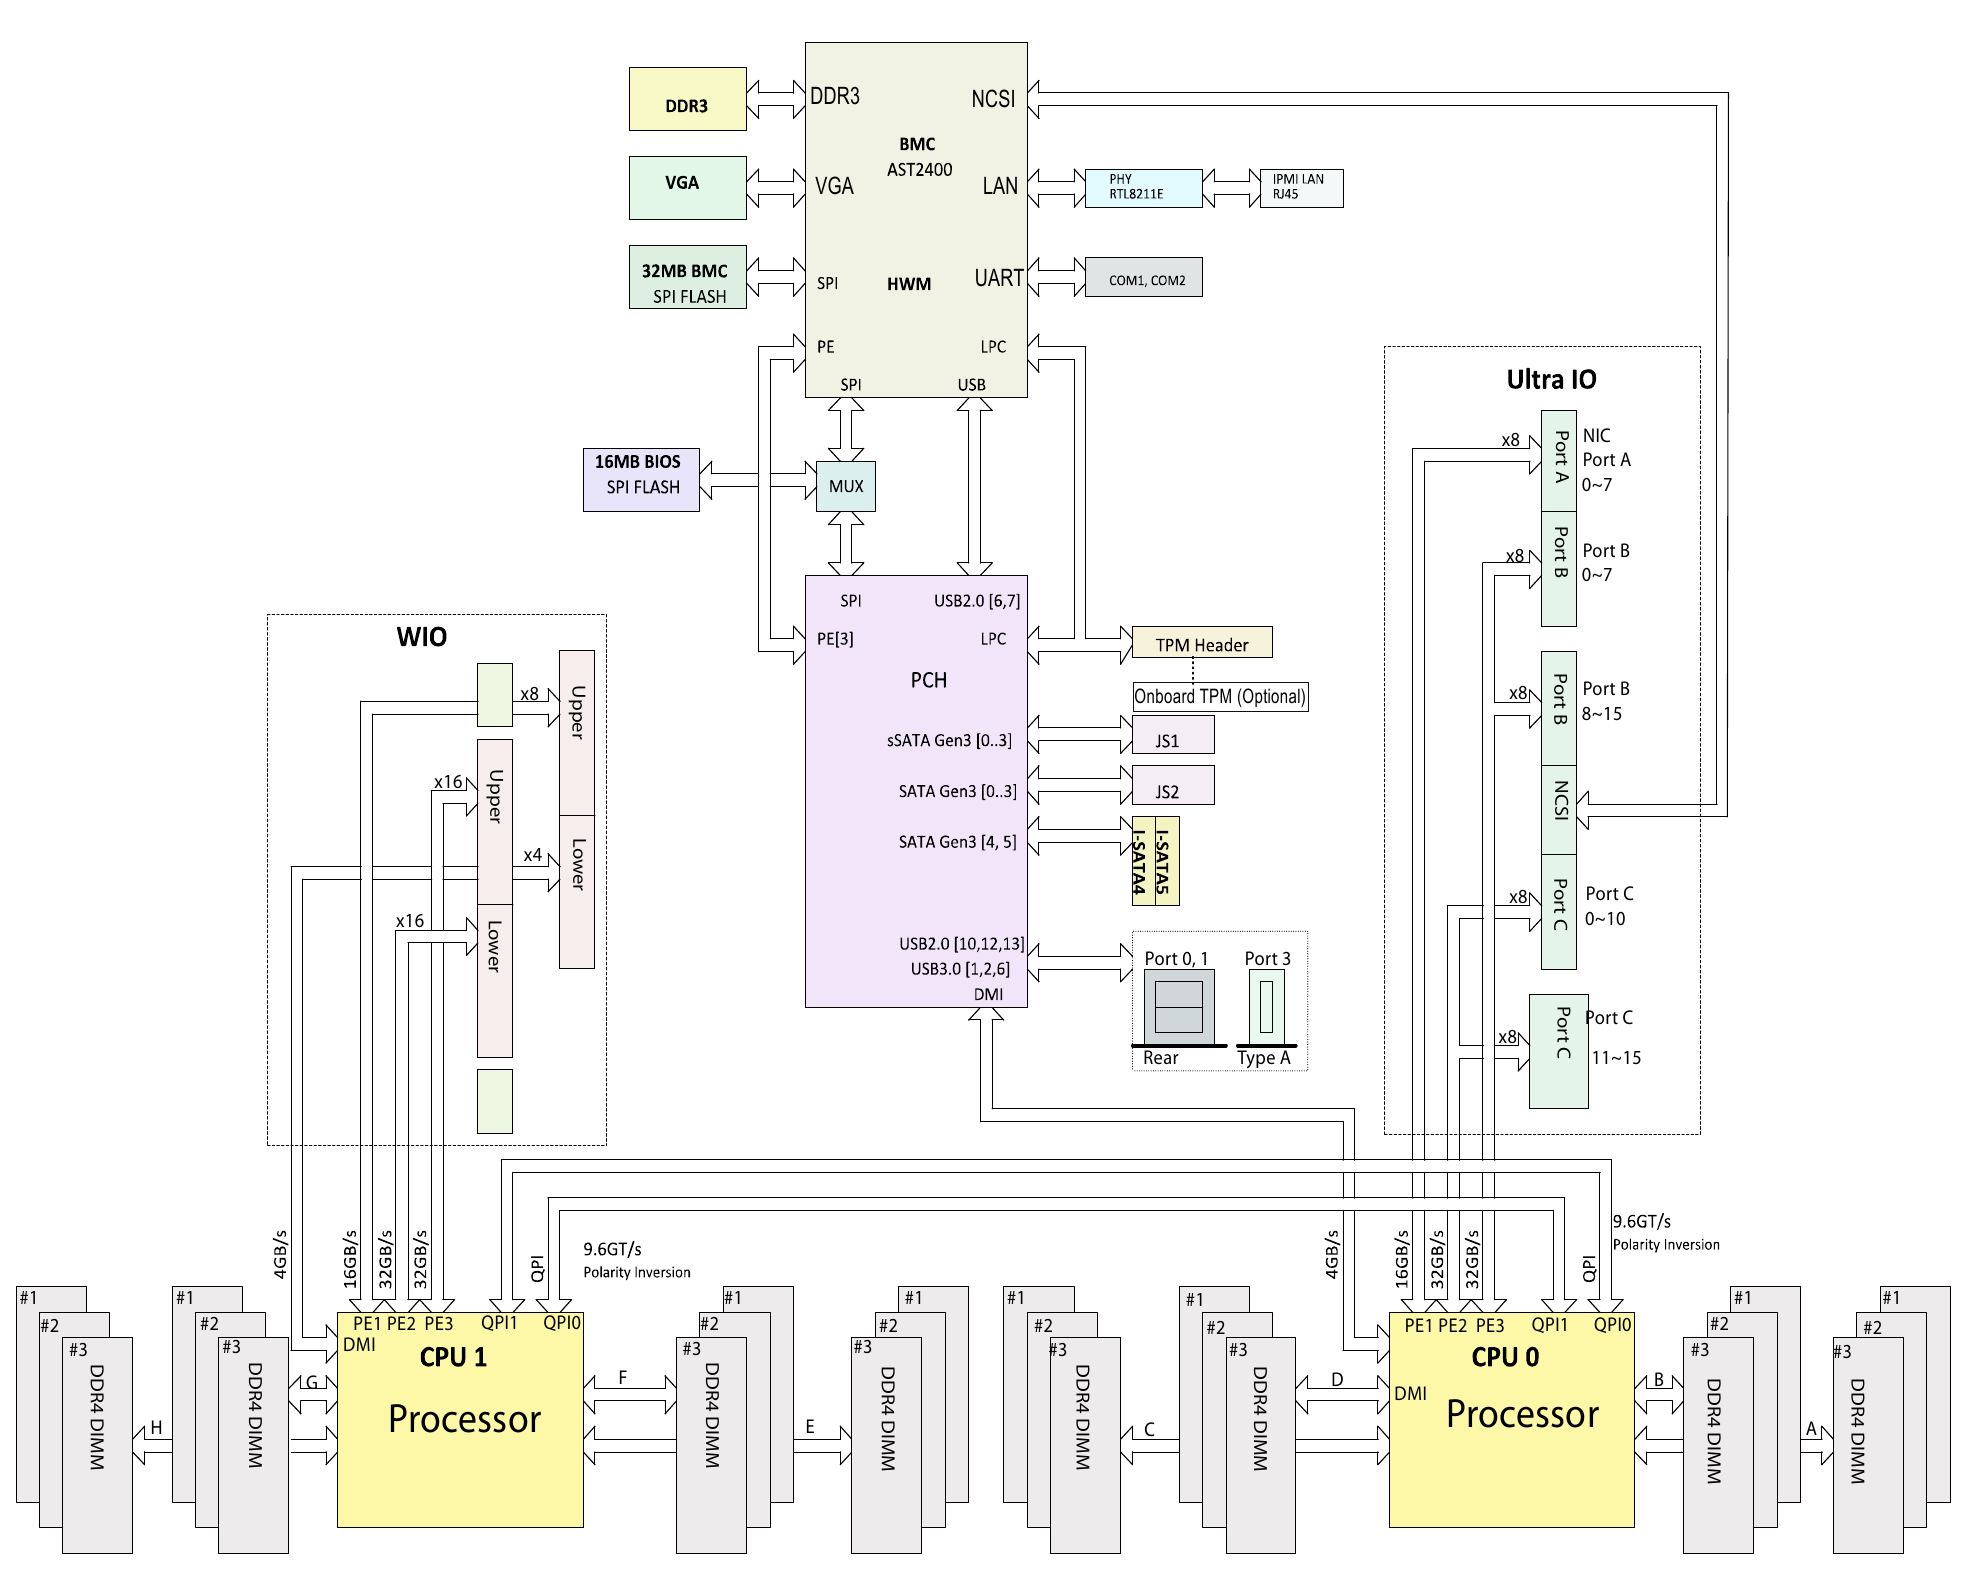
\includegraphics[width=15cm,keepaspectratio]{fig/supermicro-x10drui.png}
	\caption{Supermicro motherboard's block diagram}
	\label{fig:setup-supermicro-board}
\end{figure}

The server was put to the same rack as the Spirent hardware generator.
A pair of 40GBASE-SR4 multimode fiber cables with QSPF connectors
was used to connect Spirent with the Mellanox ConnectX-3 EN adapter.

IPv4 addresses from 192.0.2.0/24 (TEST-NET-1) block were assigned~\cite{rfc5737}.
IPv6 addresses from 2001:db8::/32 range were assigned.
Addresses within these blocks should not appear on the public Internet~\cite{rfc3849}.
Figure~\ref{fig:addressing-scheme} shows the addressing scheme used for the measurements.
\begin{figure}[H]
	\centering
	
\includegraphics[width=13.5cm,keepaspectratio]{fig/net-setup.png}
	\caption{Addressing scheme}
	\label{fig:addressing-scheme}
\end{figure}



%Enable IPv4 packet forwarding:
%echo 1 > /proc/sys/net/ipv4/ip\_forward


%ip neigh add 1.0.0.2 lladdr f4:52:14:5e:6c:71 dev enp6s0d1
%ip neigh add 2.0.0.2 lladdr f4:52:14:5e:6c:70 dev enp6s0

%ip addr add 1.0.0.1/24 broadcast 1.0.0.255 dev enp6s0d1
%ip addr add 2.0.0.1/24 broadcast 2.0.0.255 dev enp6s0


%Load BGP routes:
%\begin{lstlisting}
%Basic info: size of leaf: 40 bytes, size of tnode: 40 bytes.
%Main:
        %Aver depth:     2.43
        %Max depth:      8
        %Leaves:         503308
        %Prefixes:       538739
        %Internal nodes: 114430
          %1: 58725  2: 26171  3: 14808  4: 7316  5: 4239  6: 2103  7: 1065  8: 2  17: 1
        %Pointers: 995798
%Null ptrs: 378061
%Total size: 61373  kB
%\end{lstlisting}


%=========================================================================
% (c) 2014, 2015 Josef Lusticky

\section{Software and firmware}
Base CentOS 7 was installed on the server.
The operating system features Linux kernel based on version 3.10 -
the installed version is 3.10.0-123.20.1.el7.x86\_64.
The operating system was updated with all updates available as of 1st May 2015.
The upstream kernel version 4.0.2 was additionally installed from the ELRepo repository~\cite{elrepo-kernel-ml}.

The Linux kernel detects the Mellanox ConnectX-3 EN card automatically and loads the mlx4\_core and mlx4\_en module.
The mlx4\_core module prints the detected PCI-Express link parameters to the kernel's message buffer.
The buffer can be viewed using the {\it{dmesg}} utility and its partial output is shown bellow:
\begin{lstlisting}[language=TeX]
mlx4_core 0000:06:00.0: PCIe link speed is 8.0GT/s, device supports 8.0GT/s
mlx4_core 0000:06:00.0: PCIe link width is x8, device supports x8
\end{lstlisting}
The mlx4\_core module further registers interrupts and prints the assigned IRQ numbers for each queue
to the kernel's message buffer:
\begin{lstlisting}[language=TeX]
mlx4_core 0000:06:00.0: irq 61 for MSI/MSI-X
mlx4_core 0000:06:00.0: irq 62 for MSI/MSI-X
...
mlx4_core 0000:06:00.0: irq 90 for MSI/MSI-X
\end{lstlisting}

The driver uses either MSI or MSI-X feature of the PCI-Express bus, as described in section~\ref{sec:40gbe-throughput}.
The MSI-X feature is used automatically if the system supports it, otherwise the adapter uses MSI.
The {\it{lspci -vv}} command can be used to check whether MSI-X is used.
Listing~\ref{lst:setup-lspci} shows partial output of lspci for the Mellanox ConnectX-3 EN adapter.
The MSI-X capability is followed by an Enable flag which is followed with either "+" (enabled)
or "-" (disabled).
Listing~\ref{lst:setup-lspci} shows that the system supports MSI-X and the adapter is configured to use it.
\begin{lstlisting}[language=TeX,label={lst:setup-lspci},caption={Partial output of lspci -vv for Mellanox ConnectX-3 EN}]
06:00.0 Ethernet controller: Mellanox Technologies MT27500 Family [ConnectX-3]
		...
		Capabilities: [9c] MSI-X: Enable+ Count=128 Masked-
				...
				LnkCap: Port #8, Speed 8GT/s, Width x8, ASPM L0s, Exit Latency L0s unlimited, L1 unlimited
				...
\end{lstlisting}

Apart from the NIC driver, the Mellanox ConnectX-3 adapter uses its own proprietary firmware.
The firmware was updated to version 2.32.5100, which is the latest version available as of 10th January 2015.
The firmware is not part of the Linux kernel and its update procedure is described in appendix~\ref{app:firmware}.


%=========================================================================
% (c) 2014, 2015 Josef Lusticky

\section{Spirent configuration}
Custom iMix, named AMS-IX, was configured acording to the AMS-IX statistics described in section~\ref{sec:analysis-metodology}.
Figure~\ref{fig:setup-amsix-imix} shows the configuration window for custom iMix definiton.
One device was configured on each interface and it was assigned IPv4 and IPv6 adddress, as described in section~\ref{sec:setup-hardware}.
The "Respond to ping" option was enabled to test the connection.
Two traffic patterns were configured - one for IPv4 traffic and the other for IPv6 traffic. %TODO - pattern
\begin{figure}
	\centering
	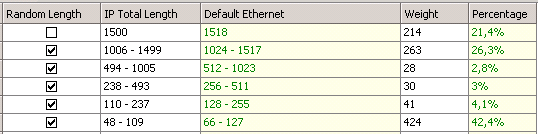
\includegraphics[width=14.5cm,keepaspectratio]{fig/amsix-imix.png}
	\caption{AMS-IX iMix}
	\label{fig:setup-amsix-imix}
\end{figure}

To test the routing performance of the Linux kernel with full BGP table, 
another scenario was configured.%TODO - scenarion, dopsat vetu


%=========================================================================
% (c) 2014, 2015 Josef Lusticky

\section{Server configuration}\label{sec:setup-server}
The general system configuration used by default in all measurements
consists of disabling Netfilter, disabling SELinux, changing the scaling governor, disabling rp\_filter and
configuring the IP addresses according to the scheme described in section~\ref{sec:setup-hardware}.
Additionally, the system should run no unused services - CentOS~7 runs Postfix, Avahi daemon, Polkitd, Tuned, Crond,
NetworkManger, dbus, crond, rsyslogd and auditd by default.
It is recommended to disable all of the services for the performance reasons.
Note that dbus may still be activated if required by any of the user-space application the system runs.
Beware that disabling NetworkManager may cause no network connectivity.
If the system uses DHCP to obtain IP address, the {\it{/etc/rc.local}} script can be used for this purpose.
Simply append {\it{dhclient}} to the end of the file and make the file executable by running {\it{chmod +x /etc/rc.local}},
but kill the {\it{dhclient}} daemon after it obtained IP address to avoid sending DHCP Request packets on other interfaces.
The services can be disable using {\it{systemctl}} command, as the following listing shows.
\newpage
\begin{lstlisting}
systemctl disable postfix avahi-daemon tuned crond polkit NetworkManager auditd dbus cron rsyslog
reboot
\end{lstlisting}
The {\it{ps uax}} command can be further used to list running processes on the system.
\\

The measurements were executed under the following conditions:
\\
Netfilter was disabled completely:
\begin{lstlisting}[language=TeX]
systemctl stop firewalld
systemctl disable firewalld  # do not execute firewalld on boot
\end{lstlisting}
SELinux was disabled by changing the SELINUX variable to {\it{disabled}} in /etc/sysconfig/selinux
(default is {\it{Enforcing}}). The system must reboot to apply:
\begin{lstlisting}
vi /etc/sysconfig/selinux
	SELINUX=disabled
reboot
\end{lstlisting}
The scaling governor was changed for each CPU to {\it{performance}} (default is {\it{powersave}}):
\begin{lstlisting}
echo performance | tee /sys/devices/system/cpu/cpu[0-9]*/cpufreq/scaling_governor
\end{lstlisting}
The rp\_filter was disabled on all interfaces (it should be disabled at least on the forwarding interfaces):
\begin{lstlisting}[language=TeX]
echo 0 | tee /proc/sys/net/ipv4/conf/*/rp_filter
\end{lstlisting}
It is suggested to disable the rp\_filter at boot time by putting the following lines to the {\it{/etc/sysctl.conf}} file:
\begin{lstlisting}[language=TeX]
net.ipv4.conf.all.rp_filter=0
net.ipv4.conf.default.rp_filter=0
net.ipv4.conf.lo.rp_filter=0
net.ipv4.conf.enp129s0.rp_filter=0        # forwarding interface 1
net.ipv4.conf.enp129s0d1.rp_filter=0      # forwarding interface 2
\end{lstlisting}
IPv6 was enabled on all interfaces (it must be enabled at least on the forwarding interfaces):
\begin{lstlisting}
echo 0 > /proc/sys/net/ipv6/conf/all/disable_ipv6
\end{lstlisting}
IPv4 forwarding was enabled:
\begin{lstlisting}
echo 1 > /proc/sys/net/ipv4/ip_forward
\end{lstlisting}
IPv6 forwarding was enabled on all interfaces (it must be enabled at least on the forwarding interfaces):
\begin{lstlisting}
echo 1 > /proc/sys/net/ipv6/conf/all/forwarding
\end{lstlisting}
IPv4 neighbours were set:
\begin{lstlisting}
ip neigh add 192.0.2.2 lladdr 00:10:94:00:00:01 dev enp6s0d1
ip neigh add 192.0.2.6 lladdr 00:10:94:00:00:02 dev enp6s0
\end{lstlisting}
IPv6 neighbours were set:
\begin{lstlisting}
ip -6 neigh add 2001:db8:1::2 lladdr 00:10:94:00:00:03 dev enp6s0d1
ip -6 neigh add 2001:db8:2::6 lladdr 00:10:94:00:00:04 dev enp6s0
\end{lstlisting}
IPv4 addresses were assigned:
\begin{lstlisting}
ip addr add 192.0.2.1/30 broadcast 192.0.2.3 dev enp6s0d1
ip addr add 192.0.2.5/30 broadcast 192.0.2.7 dev enp6s0
\end{lstlisting}
IPv6 addresses were assigned:
\begin{lstlisting}
ip -6 addr add 2001:db8:1::1/64 dev enp6s0d1
ip -6 addr add 2001:db8:2::5/64 dev enp6s0
\end{lstlisting}

The routing performance of the upstream Linux kernel version 4.0.2 was further measured.
The ELRepo was added to available repositories and the kernel was installed.
The instructions to add the ELRepo repository are provided by the elrepo.org site.\footnote{\url{http://elrepo.org/}}
Afterwards, the {\it{kernel-ml}} package was installed:
\begin{lstlisting}
yum --enablerepo=elrepo-kernel install kernel-ml
\end{lstlisting}
The kernel can be set as default in the bootloader configuration.
The following command prints all available kernels on the system:
\begin{lstlisting}[language=TeX]
grep "submenu\|^\menuentry" /boot/grub2/grub.cfg | cut -d "'" -f2
	CentOS Linux, with Linux 4.0.2-1.el7.elrepo.x86_64
	CentOS Linux, with Linux 3.10.0-123.13.1.el7.x86_64
	CentOS Linux, with Linux 0-rescue-f8351e2baaac42a285a6443a1f777333
\end{lstlisting}
The 4.0.2 kernel can be set as default by changing the configuration of grub2:
\begin{lstlisting}[language=TeX]
grub2-set-default 'CentOS Linux, with Linux 4.0.2-1.el7.elrepo.x86_64'
\end{lstlisting}

The routes announced in public BGP were imported to the kernel's FIB to perform additional measurements.
Appendix~\ref{app:bgp} describes the step-by-step instructions on how to obtain the BGP table and import it to the FIB.
Any additional system settings for a particular measurement are described next to the result.

